\documentclass{beamer}
\usepackage{amssymb}
\usepackage{textcomp}
\usepackage{amsfonts}
\usepackage{amsmath}
\usepackage{graphicx}
\usepackage{xcolor}
\usepackage{verbatim}
\usepackage{graphicx}
\usepackage{float}
\usepackage{afterpage}
\usepackage{amsmath}
\usepackage{makecell}
\allowdisplaybreaks
\usepackage{bm}
\usepackage{setspace}
\usepackage{natbib}
\usepackage[utf8]{inputenc}
\usepackage[T1]{fontenc}
%\usepackage[backend=bibtex]{biblatex}
%\addbibresource{presentation.bib}
\linespread{1}
\date{}
\addtobeamertemplate{navigation symbols}{}{%
    \usebeamerfont{footline}%
    \usebeamercolor[fg]{footline}%
    \hspace{1em}%
    \insertframenumber/\inserttotalframenumber
}
\title{Semi-Markov Models with Phase-Type Sojourn Distributions, by Titman, A.C. \& Sharples L.D.}
\author{Rahul Biswas}
\institute{Department of Statistics, University of Washington, Seattle}
\begin{document}
\maketitle
\begin{frame}{Example data context}
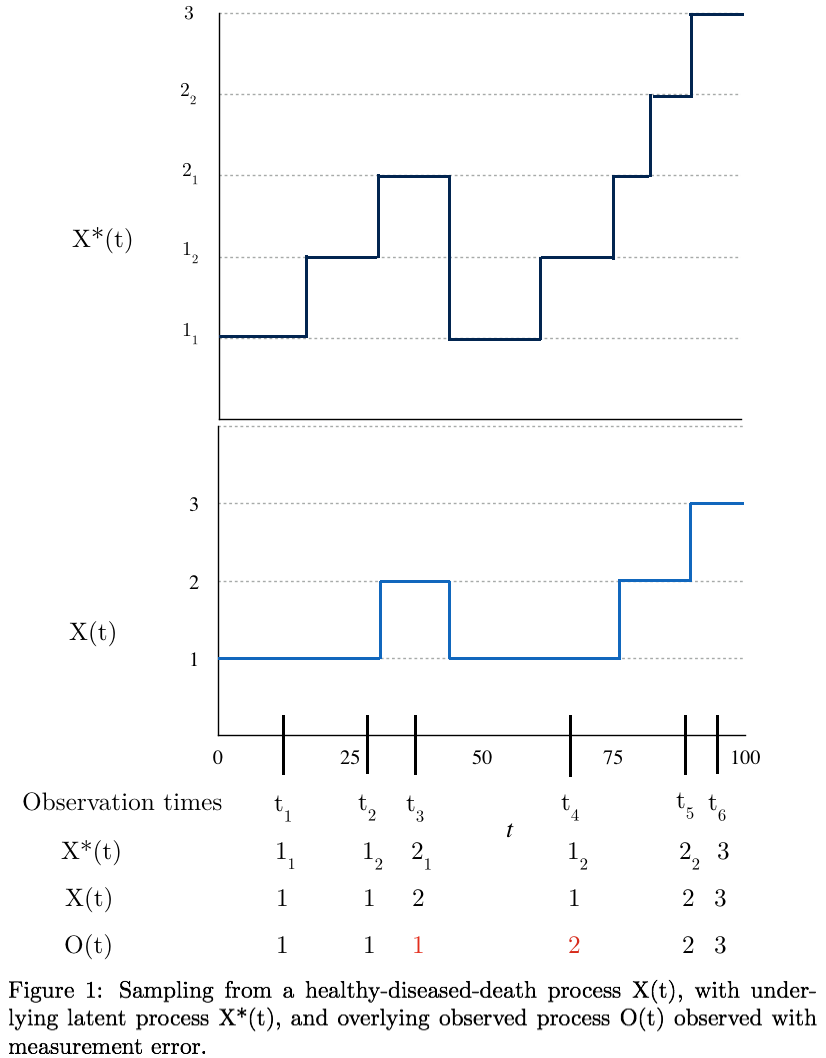
\includegraphics[scale=0.41]{figprocessAndsampling5.png}
\hspace{3mm}
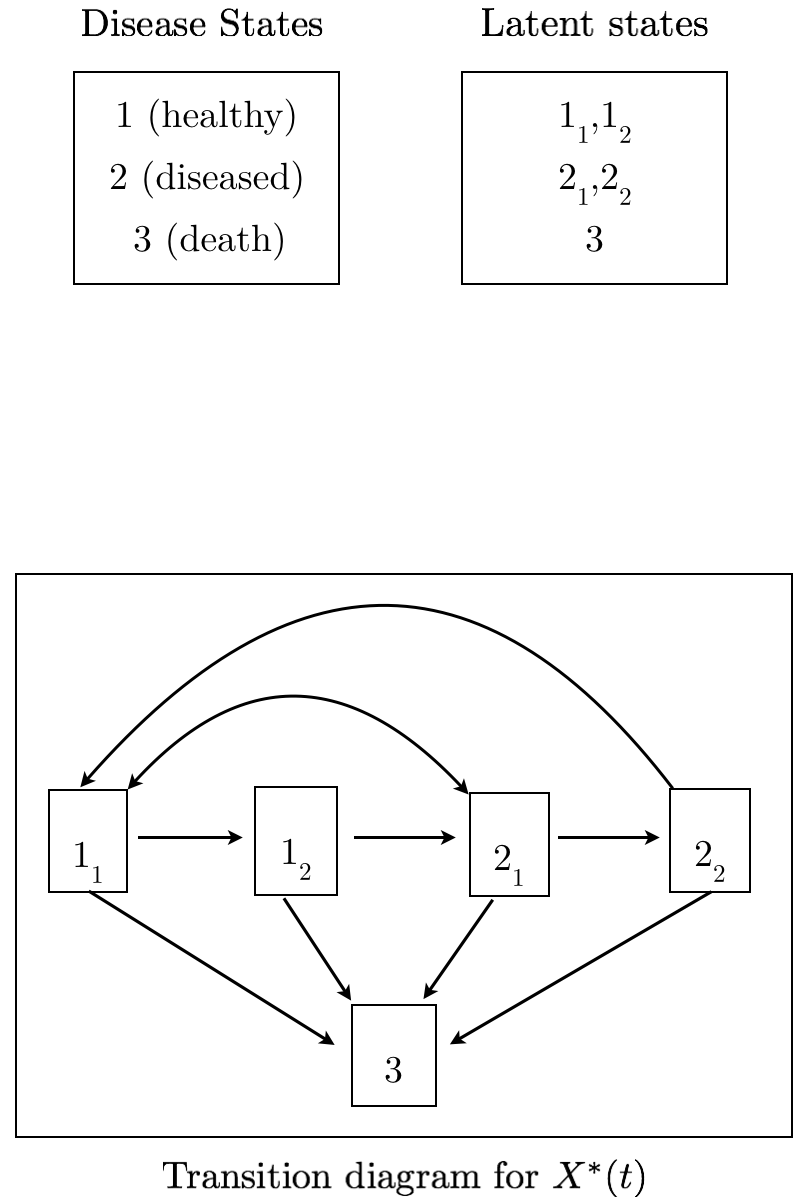
\includegraphics[scale=0.27]{datatransitions2.png}
%\caption{This is an illustration of a disease process with latent trajectory $X^*(t)$, corresponding disease trajectory $X(t)$, and misclassified trajectory $O(t)$. The three states of the disease process $X(t)$ : \{1=healthy, 2= BOS, 3=death\} with $3$ the only absorbing state. $X(t)$ has underlying latent homogeneous CTMC $X^*(t)$ with state space $S^*=\{1_1,1_2,2_1,2_2,3\}$ with $\{3\}$ an absorbing state and rest transient. $O(t)$ is the observed process which is the misclassified version of $X(t)$. States which are misclassified in this example are marked in red.}

\end{frame}
\begin{frame}{Setup and scientific objectives}
\begin{itemize}
\item Finite state continuous-time processes, with data being observed at irregularly spaced discrete time points, and no data on the trajectory of the process between these times
\vspace{4mm}
\item Assumption : Sampling mechanism from continuous time non-informative \citep{gruger1991validity}.
\vspace{4mm}
\item Scientific objectives : rate of disease onset, survival rates of patients before and after disease onset given survived for certain years after onset, extent of misclassification.
\end{itemize}
\end{frame}
\begin{frame}{Modeling Review : Homogeneous continuous time Markov chain (CTMC)}
\begin{itemize}
\item $X(t)_{t\geq 0}$ is called a continuous-time Markov chain if for any $0\leq s_0 < s_1 < \ldots <s_n < s <t+s$ and possible states $i_0,\ldots, i_n,i,j \in E$
\[
P(X_{t+s}=j|X_s =i,X_{s_n}=i_n,\ldots,X_{s_0})=P(X_{t+s}=j|X_s=i)
\]
\vspace{4mm}
\item If $P(X_{t+s}=j|X_s = i)=P(X_t = j | X_0 =i)$ for all $s\geq 0$, then $\{X_t\}$ is called homogeneous. \vspace{2mm}\\ For a homogeneous CTMC, $P(t)=\left(\left(~P(X_t = j | X_0 =i)~\right)\right)=((p_{ij}(t)))$ is called the transition probability matrix.
\end{itemize}
\end{frame}
\begin{frame}
\begin{itemize}
\item  The transition probability matrix $P(t)$ is characterized by the transition intensity matrix $\Lambda=((\lambda_{ij}))$, with \[\Lambda=\lim_{h\downarrow 0} \frac{(P(h)-I)}{h}\]\\ \vspace{5mm}
which exists when $\lim_{h \downarrow 0} P(h)=P(0)=I$. 
\vspace{8mm}
\item For a stable ($\lambda_{ii} > - \infty,\forall i$) and conservative ($\sum_{j} \lambda_{ij} =0, \forall i$) process, \[P(t) = exp(\Lambda t)\]
\end{itemize}
\end{frame}
\begin{frame}
\begin{itemize}
\item Likelihood for an individual is (under Markov  assumption) :
\[
L(\theta) = \prod_{i=1}^n p_{x_{i-1},x_i} (t_{i-1},t_i;\theta)
\] where for the individual observed states $x_0 ,\ldots, x_n$ at times (can be irregular) $t_0,\ldots,t_n$, n can be subject specific.
\end{itemize}
\end{frame}
\begin{frame}
\begin{itemize}
\item Advantage : Simple and computationally tractable
\item Disadvantage : The transition intensities are constant over time and the distribution of sojourn time in a state is always exponential, these assumptions are often unrealistic.
\end{itemize}
\end{frame}
\begin{frame}{Inhomogeneous CTMC}
Inhomogeneous CTMC is defined by the time dependent transition intensities \[\lambda_{ij}(t)=\lim_{h \downarrow 0} \frac{P(X(t+h)=j|X(t)=i)}{h}\].

\begin{itemize}
\item Advantage : Transition intensities vary with respect to time since the process origin.
\item Disadvantage : For diseases often transition intensities may depend on the time spent in the current state (sojourn time), not just external time.
\item Semi-Markov models have such a property and are considered by \cite{titman2010semi} \citep{cox1965theory,mcgllchrist1991semi}.
\end{itemize}
\end{frame}
\begin{frame}{Semi-Markov Model}
\begin{itemize}
\item In a semi-Markov model the transition intensities depend on the time spent in the current state
\[
\lambda_{ij} (u) = \lim_{h \downarrow 0} \frac{P(X(t+h) = j | X(t) = i, T^* = t-u)}{h}
\] where $T^*$ denotes the time since entry into the current state.
\item In semi-Markov models the sojourn times in each state are not constrained to have exponential distributions in contrast to time homogeneous Markov models. 
\item Titman \& Sharples specify the sojourn distribution of $X(t)$ to be of Coxian phase-type (discussed later).
\end{itemize}
\end{frame}

\begin{frame}{Problems in fitting of Semi-Markov models}
\begin{itemize}
\item Likelihood is not tractable if allowing reversible transitions. \citep{chen2004semi,foucher2010flexible}
\item Allowing reversible transitions shown tractable under stringent restrictions : \\- If evenly spaced two-state recurrent model \citep{rosychuk2001semi}\\- If at least one state has exponential sojourn distribution \citep{kang2007statistical}.
\end{itemize}
\end{frame}
%\begin{frame}{Hope}
%\begin{itemize}
%\item Computational advantages in using a latent homogeneous CTMC in two-state recurrent model. (Crespi et al.; 2005)\\ State space $\{0,1,2,\ldots\}$, a subject was considered to be disease free if in state $0$ and ill otherwise.
%\item The resulting model is semi-Markov with a phase-type sojourn distribution.\\ Transition intensities depend on time since entry into a state.
%\item The likelihood can be expressed to have the same form as of a hidden Markov model (HMM). \\ Straightforward computational techniques possible.
%\end{itemize}
%\end{frame}
\begin{frame}{Titman \& Sharples (2010)}
\begin{itemize}
\item Proposed a general approach to semi-Markov modeling and fitting to panel observed processes using a latent state CTMC.
\item Each state maps to multiple latent states, which are traversed according to an underlying CTMC.
\item This framework yields rates of transition between states that depend on the duration spent in that state, yet likelihoods are analytically tractable, even for disease processes with reversible transitions.
\item The model is extended to incorporate misclassification error.
\item Methods for inference of parameters while addressing non-identifiability concerns

\end{itemize}
\end{frame}
\begin{frame}{Details of the model}
\begin{itemize}
\item $X(t)$ denotes a continuous time stochastic process with state space $\{1,\ldots, R\}$, where $t$ is time since process origin. Let $R$ be the only absorbing state. 
\item Underlying $X(t)$ there is the latent homogeneous CTMC $X^*(t)$ with latent state space $\{1_1,\ldots1_{s_1}\}\cup \ldots \cup \{(R-1)_1,\ldots (R-1)_{s_{R-1}} \cup R\} $. $X(t)=r \Leftrightarrow X^*(t) \in \{r_1,\ldots r_{s_r}\}$ for $r<R$ and $X(t)=R \Leftrightarrow X^*(t) =R$. 
\item The sojourn distribution of each non-absorbing state $r$ of $X(t)$ is assumed to be a $k$-phase Coxian phase-type distribution, which defined as the distribution of absorption time of a progressive CTMC with $k$ transient states and one absorbing state. 
\item The transition diagram of the underlying process is illustrated in Figure.
%\item Thus for observable state $r$, the latent process $X^* (t)$ can have the states $r_1,\ldots,r_k$,  with parameters $\lambda_{r_j} =$ the intensity for movement from $r_j$ to $r_{j+1}$, for $j=1,\ldots, k-1$, with the assumption that these latent phases for each observable state is progressive thereby all other transitions between $r_j$'s have $0$ intensity, and $\mu_{r_j s}=$, the intensity for movement out of a latent phase of $r_j$ to state $s$ with the assumption that any state $s$ is entered only at latent phase $s_1$, thereby all other intensities for transition from latent phases of $r$ to latent phases of $s$ are $0$. Figure 1 summarizes the transition diagram for transitions between latent phases of observable state r and transition out to observable state s. 

%\item $X(t)$ Semi-Markov process with state space $S=\{1,\ldots, R\}$, where $R$ is the only absorbing state. 
%\item $X^* (t)$ underlying CTMC, with state space $S^*=\{1_1,\ldots,1_k\} \cup \{2_1,\ldots,2_k\}\cup \ldots \cup \{(R-1)_1,\ldots,(R-1)_k\} \cup R$ with parameters as progressive transition intensities between phases of a state and for transition from a phase of a state to the beginning of another state, and initial distribution.
\end{itemize}
\end{frame}
\begin{frame}
\begin{figure}
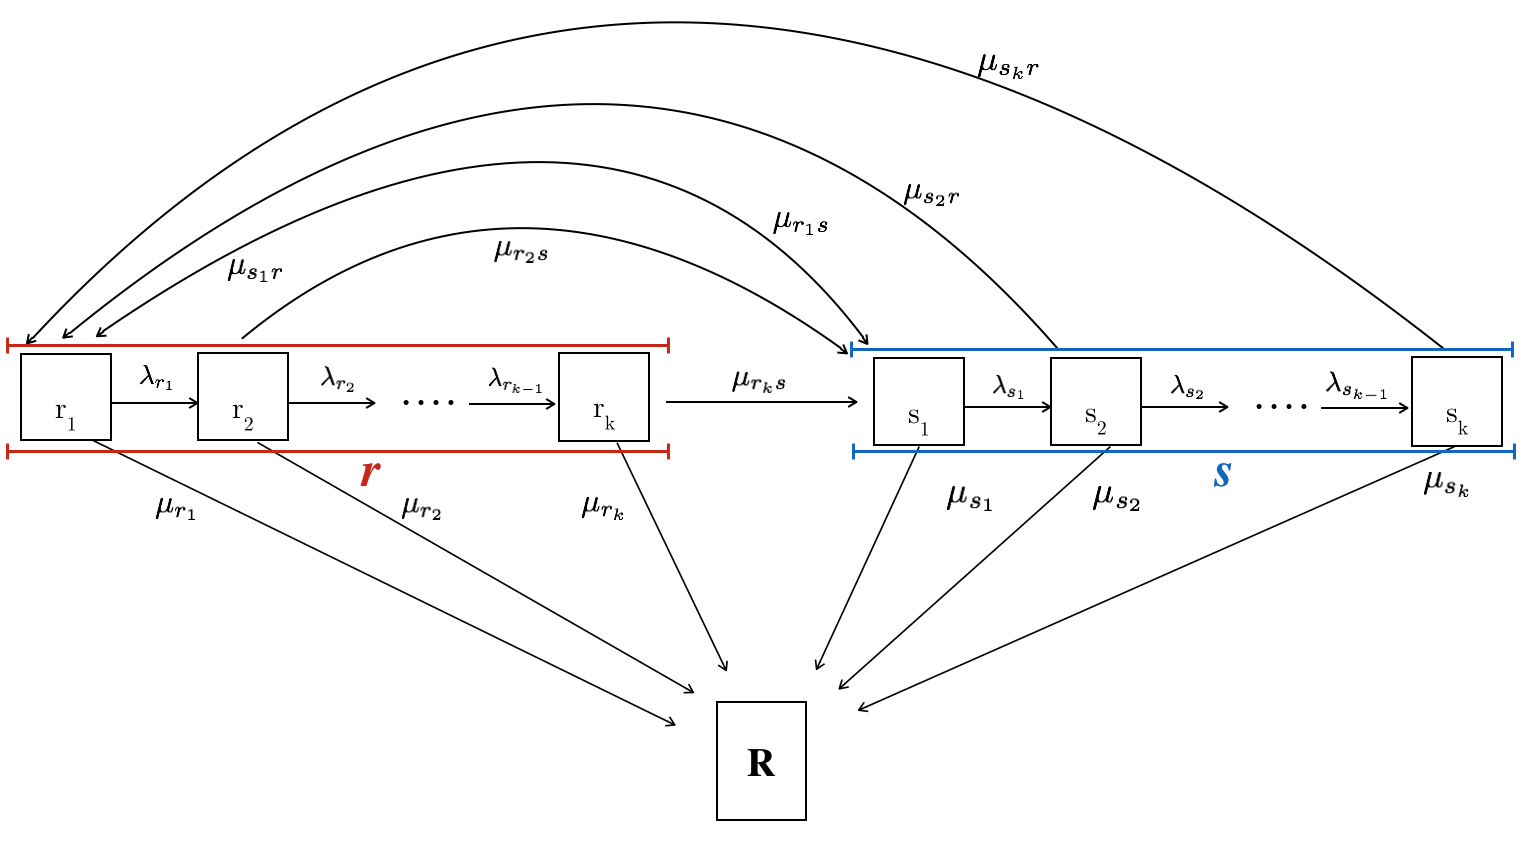
\includegraphics[scale=0.4]{coxmodelstitched2.png}
\caption{Transition diagram for the underlying latent model.}
\end{figure}
\end{frame}
\begin{frame}
\begin{itemize}
\item Advantage 1 of using phase type distributions :  generality as phase type distributions are dense in the class of all distributions with non-negative support (Neuts, 1974). 
\item Advantage 2 : Analytic tractability is ensured with density, cumulative distribution function and failure rate being matrix exponentials.
\item Disadvantage :The model may not be identifiable \citep{asmussen1996fitting}. \\ \vspace{2mm}But, typical scientifically meaningful functionals of sojourn distribution parameters like hazard function are identifiable \citep{bladt2003estimation}.
\end{itemize}
\end{frame}
\begin{frame}
\begin{itemize}
\item For greater estimability and interpretation of moving out of a state to another it is assumed that $\mu_{r_j s} = \tau_{r_j} \mu_{r_1 s} \forall s$, $\tau_{r_1}=1$. %That is rates of exiting from latent phase $r_j$ relative to $r_1$ change by the same factor irrespective of destination. 
\item It is noted that the resulting $X(t)$ is a semi-Markov process.
\item To incorporate misclassification, observed states are O(t) with misclassification probability : $e_{rs}=P(O(t)=s|X(t) =r)=P(O(t)=s|X^* (t) =r_j)= e^*_{r_j s}$ for $r,s = 1,\ldots,R$, $j=1,\ldots, k$. 
\item The process $(O(t), X^*(t))$ is a Hidden Markov Model (HMM). Thereby computational methods tailored for statistical analysis of HMM can be used for inference.
\item Since $X(t)$ is semi-Markov, the process $(O(t),X(t))$ is termed as a Hidden semi-Markov Model (HSMM).

\end{itemize}
\end{frame}
\begin{frame}
Denoting $o_0,\ldots, o_{n}$ to be the sampled observations with misclassification at times $t_0,\ldots,t_{n}$ for an individual, the likelihood contribution for the individual based on the forward-backward algorithm for HMM can be expressed as follows.

\[
L=\pi \bm{M}_1^* \bm{M}_2^* \ldots \bm{M}_{n}^* \bm{1}
\]
where $\bm{M}_i^*$ is a $\{k(R-1) +1\} \times \{k(R-1) +1\}$ matrix with $(r^*,s^*)$ entry $e^*_{s^* o_i} p^*_{r^* s^*} (t_i - t_{i-1})$ for $r^*, s^* \in S^*$, with $P^*(t)=((p^*_{r^* s^*})) = e^{\bm{\Lambda}t}$,  and, $\pi$ is the initial state distribution.

%\item $logit(\pi_2) = a_0 + a_1 1(DL)$, and $logit(e_{12})=b_0 + b_1 1(DL)$, where $1(DL)$ is the indicator of double lung transplant.
\end{frame}
\begin{frame}
\begin{itemize}
\item Quasi-Newton method due to Broyden, Fletcher, Goldfarb and Shanno (BFGS, 1970) and, Nelder and Mead's (NM, 1965) algorithm have been used to maximize likelihood and obtain point and interval estimates of the model parameters.
\item Final quantities of interest, first passage cumulative distribution function, transition probabilities, hazard rates and survival probabilities are one-dimensional functionals of the parameter vector of the latent CTMC. \vspace{0.8mm} \\Point and interval estimates transferred using Delta method.
\end{itemize}
\end{frame}

\begin{frame}{Identifiability}
\begin{itemize}
\item The presence of misclassification and HMM setup increases possibility of non-identifiability \citep{macdonald1997hidden}.
\item In fact for a HMM with two states and balanced observation times, it is not possible to simultaneously identify the misclassification probabilities and transition intensities or probabilities without putting constraints, for instance that misclassification probabilities are each $<0.5$ \citep{rosychuk2003bias}.
\item In addition, the Coxian phase-type structure induces non-identifiability.
\item The model parameters have been appropriately constrained here by $\mu_{r_j s}=\tau_{r_j } \mu_{r_1 s}$ to embetter on that. 
%\item Also, profile-likelihood plots and unimodal appearance of likelihood noted by authors as checks for ensuring optima is global.
\end{itemize}
\end{frame}

\begin{frame}{Hypothesis tests}
\begin{itemize}
\item Markov vs phase-type semi-Markov model : Due to identifiability problems, likelihood ratio tests may not have asymptotic $\chi^2$ distribution. \\ \vspace{2mm} Authors considered an aptly penalized likelihood (based on \cite{chen2001modified}) instead.

\item Goodness of fit : \cite{aguirre2002pearson} proposed a Pearson-type goodness of fit test for Markov models.\\  \vspace{2mm} It was not applicable if there was an absorbing state. \\  \vspace{2mm}\cite{titman2008general} proposed a modification applicable in such scenario for MMs as well as HMMs, which has been used in the present paper.
\end{itemize}
\end{frame}

\begin{frame}{BOS dataset}
\begin{itemize}
\item Bronchiolitis obliterans syndrome (BOS) is the irreversible progressive narrowing of bronchiolar lumens and airflow obstruction \citep{todd2011bronchiolitis}, leading to impaired lung function.
\item It is recorded to affect a majority of lung transplant recipients and is the principal factor limiting long-term transplant survival.
\item The dataset includes 364 post-lung-transplant patients who received transplants at Papworth Hospital between 1984 and 2006, with 242 heart-lung transplant and 122 both-lung trasnplant patients. 
\item Patients were scheduled to for visit at 9 months, 12 months, after that at 6 month intervals, but actual visit times were highly irregular, and can be of different number
\end{itemize}
\end{frame}

\begin{frame}
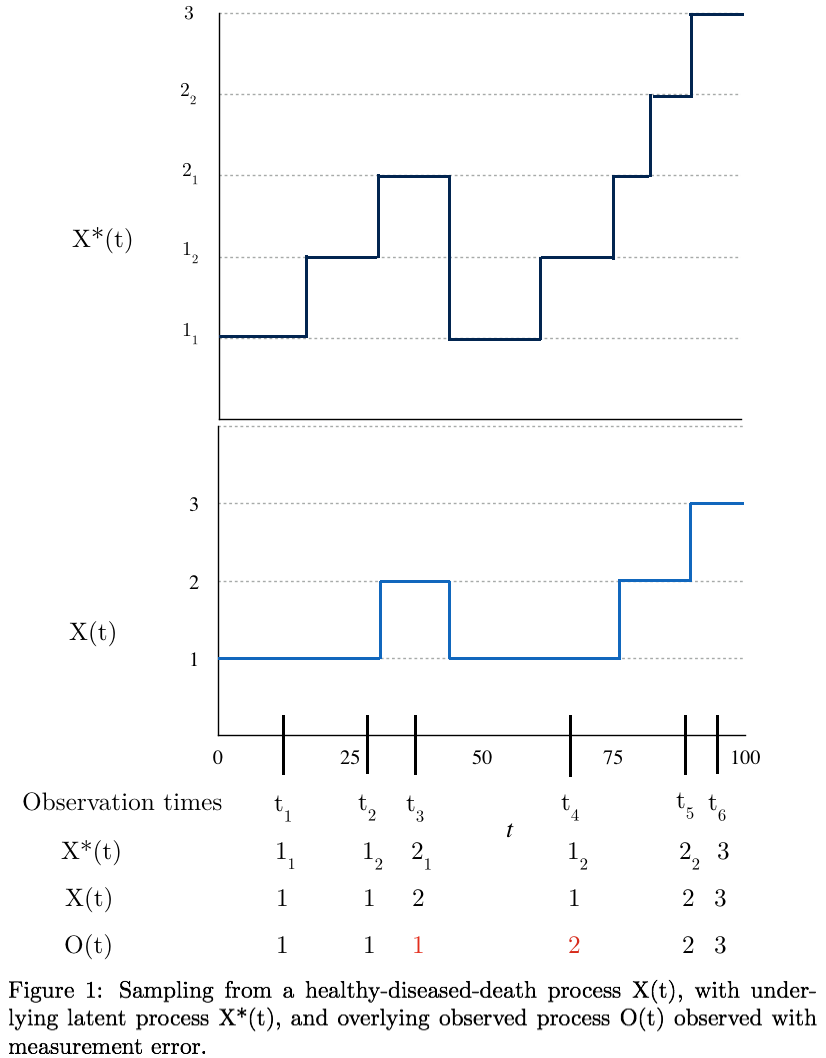
\includegraphics[scale=0.4]{figprocessAndsampling5.png}
\hspace{3mm}
\includegraphics[scale=0.25]{datatransitions.png}
\end{frame}


\begin{frame}
\begin{itemize}
\item $\pi_{1_2}=\pi_{2_2}=\pi_3=0$
\vspace{5mm}
\item $logit(\pi_{2_1}) = a_0 + a_1 1(DL)$, and $logit(e_{12})=b_0 + b_1 1(DL)$, where $1(DL)$ is the indicator of double lung transplant.
\end{itemize}
\end{frame}

\begin{frame}{Computation results}
\begin{itemize}

\item Default relative convergence tolerance of 'optim' ($10^{-8}$) and number of likelihood evaluations limited at $2500$ for both Broyden, Fletcher, Goldfarb and Shanno (BFGS, 1970), and, Nelder and Mead's (NM, 1965) algorithm.

\item To check for global optimum and run-time, we computed the MLE for each algorithm with 20 random starting values from independent Normal (mean=0,sd=0.25).
\end{itemize}
\end{frame}
\begin{frame}
\begin{figure}[t]\label{fig:comp_ll}
\centering
\includegraphics[scale=0.26]{comp_ll_timetaken.pdf}
\caption{Runtime and attained LL using BFGS and NM algorithm to fit the BOS data, using 20 random starting values for each.}
\end{figure}
\end{frame}
\begin{frame}
\begin{itemize}
\item The median run-time of the HSMM optimization over 30 runs was 4394.47 seconds for the NM and 2676.755 seconds for the BFGS algorithm.
\item NM was particularly poor at converging to either a local or global maxima and reached the iteration limit 16/20 times. BFGS converged to a local maxima in 17/20 trials.
\item Presence of multiple local maxima where the algorithm converged, and, non-identifiability that is, different parameters leading to approximately same likelihood has been recorded in this process.
\end{itemize}
\end{frame}

\begin{frame}
\begin{table}[t]
\centering
\caption{This is a demonstration of non-identifiability of the likelihood for the BOS dataset. Two different parameter sets lead to approximately the same likelihood.}\vspace{4mm}
\resizebox{\columnwidth}{!}{%
\begin{tabular}{cccccccccccccc}
\hline
\multicolumn{8}{c}{Transition intensities} & \multicolumn{3}{c}{Emission probabilities} & \multicolumn{2}{c}{Initial distribution} & \\ 

$1_1 \rightarrow 1_2$ & $1_1\rightarrow 2_1$ & $1_1\rightarrow 3$ & $\tau_{1_2}$ & $2_1 \rightarrow 2_2$ & $2_1 \rightarrow 1_1$ & $2_1\rightarrow 3$ & $\tau_{2_2}$ & e(BOS,healthy) & \multicolumn{2}{c}{e(Healthy, BOS)} & \multicolumn{2}{c}{$\pi(\mbox{BOS}_1)$}  & $-LL$\\
\multicolumn{8}{c}{} & & Heart lung & Double lung & Heart lung & Double lung & \\
\hline
0.12 &  0.34 &  0.00 & 0.27 & 36.25 &  1.24 &  8.51 &  0.03 &  0.01 &  0.51 &  0.80 & 0.53 & 0.56 & 1615.143\\
0.26 & 0.35 & 0.03  & 0.37 & 5.11 & 0.18 & 1.31 & 0.16 & 0.01 & 0.51 & 0.79 & 0.52 & 0.77 & 1615.261\\
\hline
\end{tabular}
}
\vspace{2mm}
\end{table}
\end{frame}

\begin{frame}{BOS results}
\begin{table}[b!]
\centering
\resizebox{\columnwidth}{!}{%
\begin{tabular}{ccccccc}
\hline
Intensiy rates & \thead{Transition\\ i} & \thead{\\j} & HMM point estimate & HMM 95\% CI & HSMM point estimate & HSMM 95\% CI\\
\hline
& $1_1$ & $1_2$ & & & 0.40 & (0.11,0.48) \\
& $1_1$ & $2_1$ & 0.12  & (0.09,0.15) & 0.38 & (0.27,0.55)\\
& $1_1$ & $3$ & 0.04 & (0.03,0.07) & 0.01 & (0.00,0.026)\\
& $1_2$ & $2_1$ & & & 0.17 & (0.12,0.25)\\
& $1_2$ & $3$ & & & 0.01 & (0.00,0.12 )\\
& $2_1$ & $2_2$ & & & 7.97 & (0.19,36.03)\\
& $2_1$ & $1_1$ & 0.03 & (0.01,0.13) & 1.00 & (0.18,5.72)\\
& $2_1$ & $3$ & 0.25 & (0.20,0.30) & 2.41 & (0.11,5.76)\\
& $2_2$ & $1_1$ &  &  & 0.04 & (0.02,0.08)\\
& $2_2$ & $3$ &  &  & 0.21 & (0.16,0.28)\\
\hline
\hline
Emission & e(Healthy, BOS) & Heart Lung & 0.50 & (0.50,0.50) & 0.507 & (0.506,0.507)\\
& & Double Lung & 0.50 & (0.50,0.50) & 0.77 & (0.71,0.83)\\
& e(BOS, Healthy)& & 0.526 & (0.524,0.527) & 0.50 & (0.5019,0.5021)\\
\hline
\hline
Initial distribution & $\pi(\mbox{BOS}_1)$ & Heart Lung & 0.50 & (0.50,0.50) & 0.523 & (0.522,0.530)\\
& & Double Lung & 0.50 & (0.50,0.50) & 0.70 & (0.64,0.78)\\
\hline
\hline
- Log-likelihood & & & \multicolumn{2}{c}{-2533.91} & \multicolumn{2}{c}{-1619.88}\\
BIC & & & \multicolumn{2}{c}{5120.89} & \multicolumn{2}{c}{3316.41}\\
No. pars & & & \multicolumn{2}{c}{9} & \multicolumn{2}{c}{13}\\
\hline
\end{tabular}
}
\vspace{2mm}
\caption{Maximum likelihood estimation for model intensity rates, emission probabilities, and initial probabilities based on hidden Markov and phase-type HSMMs.}

\end{table}
%\begin{table}
%\centering
%\caption{Parameter estimates for HMM and phase-type HSMMs for BOS dataset}
%\hspace{-2mm}
%\resizebox{\columnwidth}{!}{%
%\begin{tabular}{|c|cc|cc|}
%\hline
%Parameter & HMM Estimate & HMM CI & HSMM Estimate & HSMM CI\\
%\hline
%$\lambda_1$ & & & 0.21 & (0.05,0.95) \\
%$\mu_{1_1 2}$ & 0.12  & (0.09,0.15) & 0.36 & (0.26,0.50)\\
%$\mu_{1_1 3}$ & 0.04 & (0.03,0.07) & 0.00 & (0.00,0.002)\\
%$\tau_{1_2}$ & &  & 0.37  & (0.21,0.65)\\
%$\lambda_2$& & & 29.00 & (0.00,82.17)\\
%$\mu_{2_1 1}$& 0.03 & (0.01,0.13) & 1.00 & (0.18,5.72)\\
%$\mu_{2_1 3}$& 0.25 & (0.20,0.30) & 7.02 & (0.79,1.94)\\
%$\tau_{2_2}$& & & 0.01 & (0.00,0.27)\\
%$e_{21}$& 0.10 & (0.07,0.15) & 0.00 & (0.00,0.03)\\
%$e_{12}^{HL}$& 0 & (0,1) & 0.02 & (0.02,0.04)\\
%$e_{12}^{DL}$& 0 & (0,1) & 0.56 & (0.42,0.68)\\
%$\pi_{2,HL}$& 0 & (0,1) & 0.09 & (0.05,0.14)\\
%$\pi_{2,DL}$& 0 & (0,1) & 0.76 & (0.19,0.72)\\
%$- LL$& -2533.91 & & -1617.978 &\\
%No. pars & 9 & & 13 &\\
%\hline
%\end{tabular}
%}
%\end{table}
\end{frame}
\begin{frame}
\begin{figure}[t!]
\centering
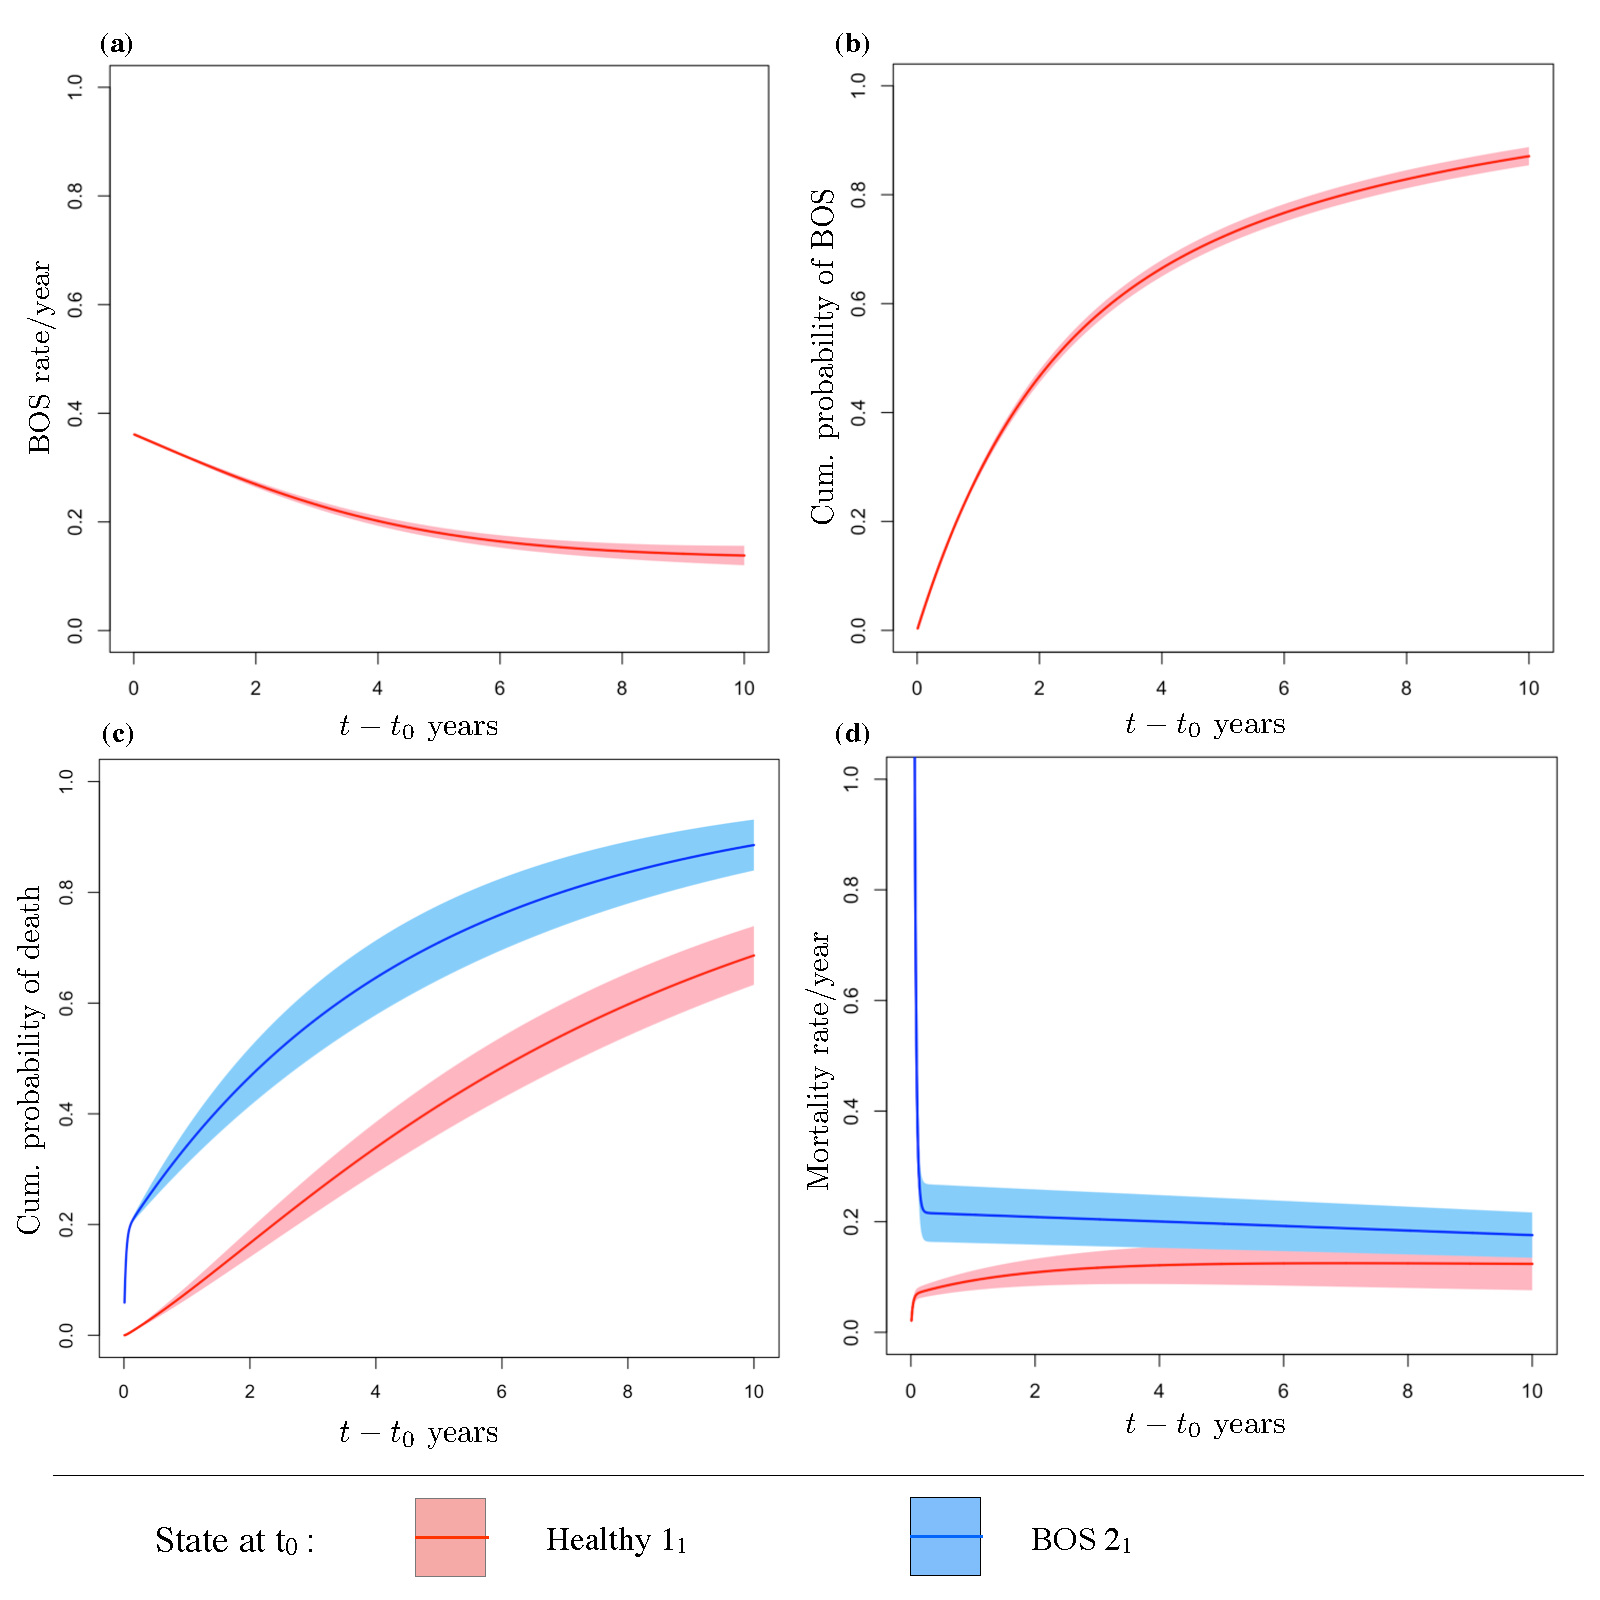
\includegraphics[scale=0.3]{4plots4.pdf}
\end{figure}
\end{frame}
\begin{frame}
\begin{itemize}
\item The model predicts that the rate of entry into the diseased states decrease with time since transplant; Initially disease rates are 35\%–40\%, and decrease to 18\% per year after 5 years
\vspace{5mm}
\item Decreasing BOS rates are agreeing with the fact that risk for experiencing infections or acute rejection episodes, which may trigger BOS development, is high at the initial period right after transplant.
\end{itemize}
\end{frame}
\begin{frame}
\begin{itemize}
\item By 2 years post transplant, about 17\% of those healthy at the beginning of the study are estimated to have died. After BOS initiation, about 66\% remain alive for 1 year, 43\% for 3 years, 29\% for 5 years.
\vspace{5mm}
\item Till before BOS onset, mortality rates are very low. After having BOS onset, mortality rates increase drastically to >50\% per year, and then decrease to 20\% after 2 years, followed by a gradual decline in rate.
\end{itemize}
\end{frame}
\begin{frame}
\begin{figure}
\centering
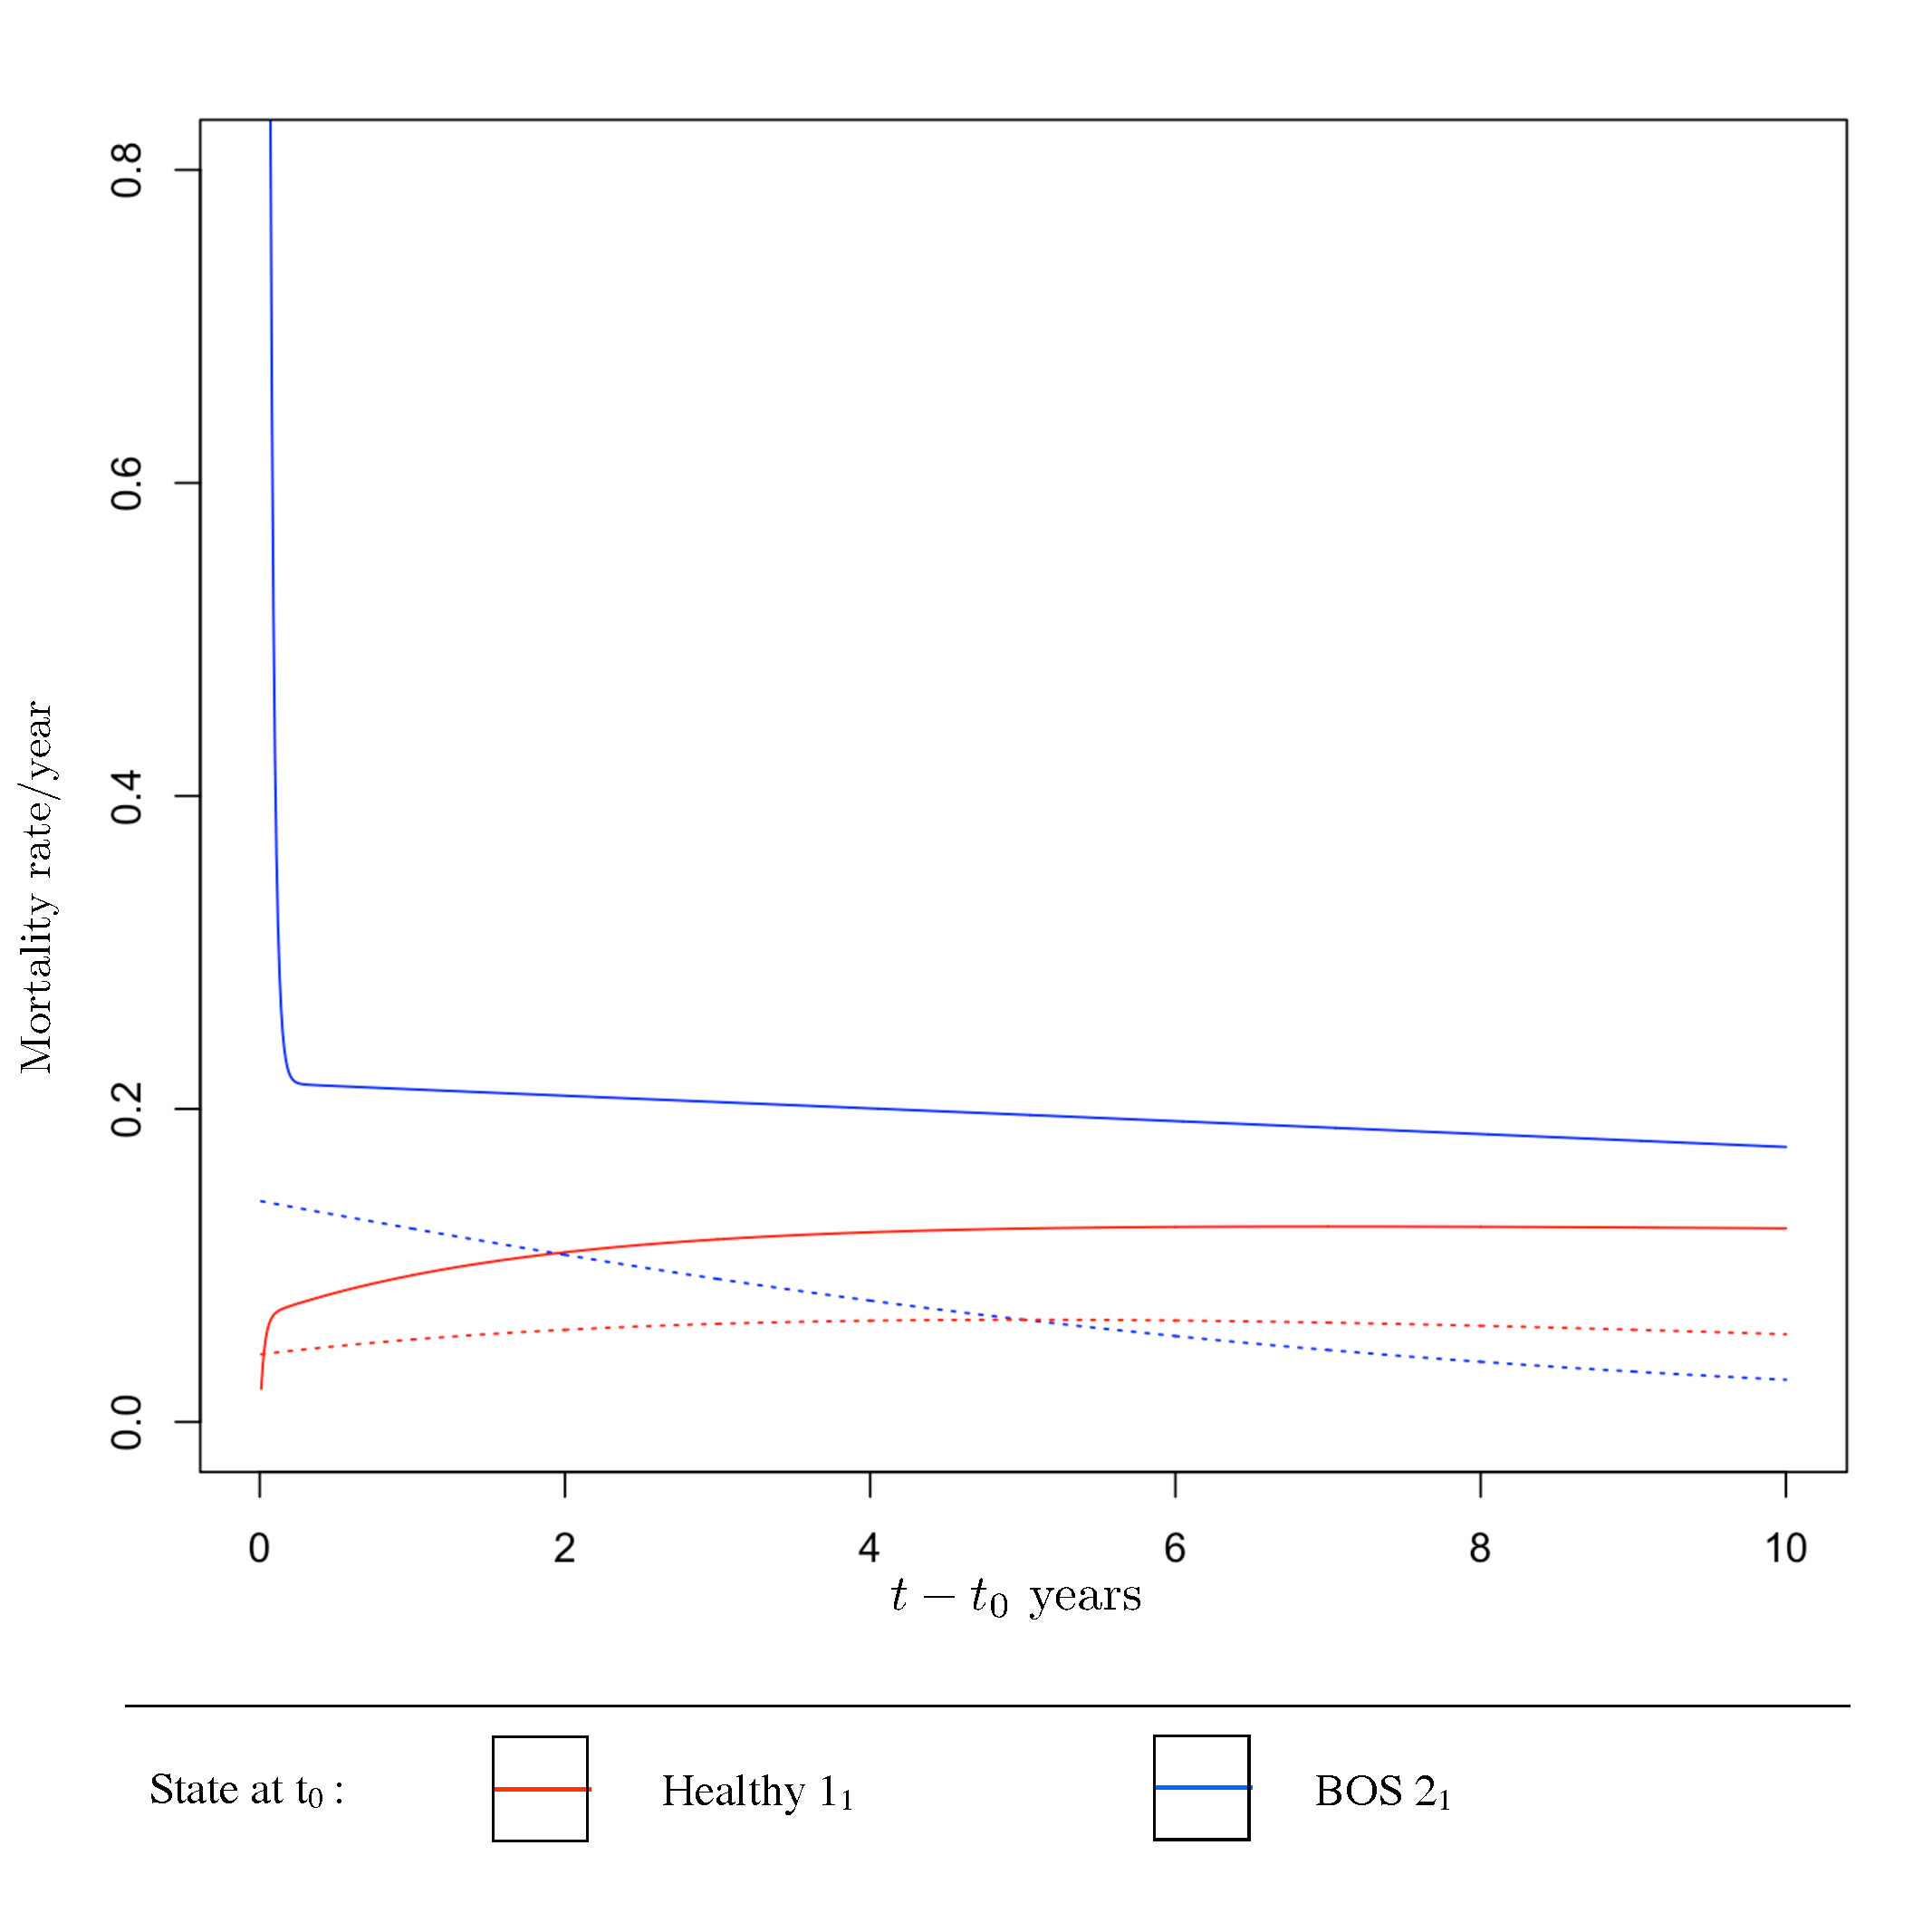
\includegraphics[scale=0.25]{mortcomp_hsmmhmm.pdf}
\caption{Unlike the HSMM model, the HMM model did not show the detailed artifacts of the disease mortality rates backed by the medical literature.}
\end{figure}
\end{frame}
\begin{frame}{Hypothesis tests}
\begin{itemize}
\item Goodness of Fit test \citep{titman2008general} : At 95\% level, evidence in favor of good fit of the HSMM model. The statistic is recorded to have a value 31.09, which is rejected under null distribution, under which $\chi^2(32) (0.95)=46.2$ is an upper bound to the $95\%$ quantile. At level 95\%, evidence in favor of poor fit of HMM model, with test statistic being 96.81 on $\chi^2_{24}$ distribution.
\item Null hypothesis of HMM vs. alternative of HSMM (Modified likelihood ratio test based on \cite{chen2001modified}) : The value of the test statistic was 25.18. The test statistic has an approximate $\chi^2(2)$ distribution whose $95\%$ quantile is nearly $5.99$. Therefore, this shows strong evidence against the HMM model in favor of the HSMM model.
\end{itemize}
\end{frame}
\begin{frame}
\begin{itemize}
\item Biologically, BOS is an irreversible disease.
\item Yet Titman and Sharples (2010) included a BOS $\rightarrow$ healthy transition in their latent CTMC model, based on recording a likelihood ratio test in the standard CTMC HMM setup, whence there was support in favor of including a BOS $\rightarrow$ healthy transition.
\item We test whether to include BOS $\rightarrow$ healthy transition in the HSMM setup. That is we compare the null hypothesis of HSMM model with the BOS $\rightarrow$ healthy transition rate 0 versus the alternative of an HSMM model with this transition rate positive. 
\item The test statistic is 9.038. 
\item The null hypothesis is on the boundary of the parameter space; thus the distribution of the likelihood ratio test statistic is a 50:50 mixture of a chi-square with 1 df and a point mass at zero \cite{self1987asymptotic}. 
\item The p-value for the LR test statistic was 0.0013, which is evidence in favor of including the reversible transition.
\end{itemize}
\end{frame}
%\begin{frame}[allowframebreaks]
 % \frametitle{References}
  %\nocite{*}
  %\printbibliography
 %\end{frame}
% \begin{frame}
% \item 
% \item Lange \& Minin (2013) proposed an EM algorithm for this setup, which is efficient and robust and demonstrated to have outperformed optimization methods, like Nelder-Mead and BFGS, for a slightly different BOS dataset.
% \end{frame}
 \begin{frame}{Summary}
\begin{itemize}
\item Modeling panel observed data by a Semi-Markov model with latent homogeneous CTMC, phase-type sojourn distribution
\item Incorporating misclassification error
\item A general approach for inference of parameters addressing non-identifiability and testing significance and fit.
\item Application of the method to assess development of bronchilitis obliterans syndrome in post-lung-transpantation patients, making comparison with standard HMM.
\end{itemize}
\end{frame}
%\begin{frame}
%\begin{itemize}
%\item Uneven observation times, and of different number motivating usage of CTMC (why? - vlad book)
%\item Transition intensities of the process depend on time since entry into a state making the process
%\item Inference of parameters addressing non-identifiability
%\item Application of the method to assess development of bronchilitis obliterans syndrome in post-lung-transpantation patients, making comparison with existing popular method.
%\end{itemize}
%\end{frame}
\begin{frame}
\begin{center}
\Huge Thank you!
\end{center}
\end{frame}
\begin{frame}[allowframebreaks]
\frametitle{References}
\bibliographystyle{apalike} 
\bibliography{presentation.bib}
%\printbibliography
\end{frame}
\end{document}